\documentclass[tikz]{standalone}
\usetikzlibrary{bayesnet, arrows.meta}

\begin{document}
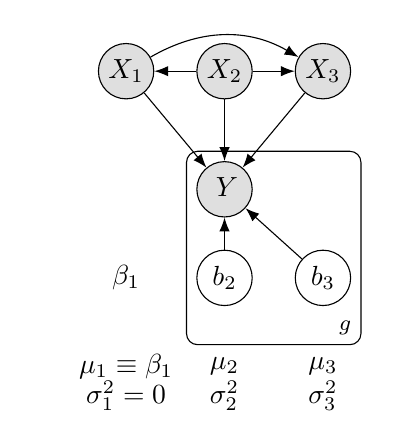
\begin{tikzpicture}


% GLOBAL SETTINGS
\newcommand{\p}{3}
\newcommand{\Xstyle}{obs}
\newcommand{\Bstyle}{latent}
\newcommand{\Betastyle}{}
\newcommand{\mybeta}{\(\beta_1\)}

% SHARED CODE
\newlength{\xdist}
\setlength{\xdist}{1.25cm}
\newlength{\ydist}
\setlength{\ydist}{1.5cm}
\pgfkeys{/tikz/every path/.style={->, -{Latex[length=5pt]}}} % draw arrowheads
% X
\path (-2\xdist,\ydist) foreach \j in {1,...,\p} {
++(\xdist,0) node[\Xstyle] (X\j) {\(X_\j\)}
+(0,-1.75\ydist) coordinate (b\j) 
};
% beta
\path (-2\xdist,\ydist) foreach \j in {2,...,\p} {
(b\j) node[\Bstyle] (B\j) {\(b_{\j }\)}
};
\node[\Betastyle] (B1) at (b1) {\mybeta};
% helper coordinates
\path
(b1) +(-0.6\xdist,-0.0\ydist) coordinate (bL)
(b\p) +(+0.6\xdist,-0.0\ydist) coordinate (bR) ;
% Y
\node[obs] (Y) at (0,0) {\(Y_{}\)};



\path (-2\xdist,\ydist) foreach \j in {1,...,\p} {
(b\j) +(0,-0.75\ydist) coordinate (m\j) 
(b\j) +(0,-1.0\ydist) coordinate (c\j) 
%(b\j) +(-0.5\xdist,-1.5\ydist) coordinate (n\j) 
%(b\j) +(0\xdist,-1.75\ydist) coordinate (d\j) 
};

\path foreach \j in {2,...,\p} {
(c\j) node (C\j) {\(\sigma^2_{\j}\)}
(m\j) node (M\j) {\(\mu_{\j}\)}
%(d\j) node (D\j) {\(\mu_{\j}\)}
};

\path (m1) node (M1) {\(\mu_1 \equiv \beta_1\)};
\path (c1) node (C1) {\(\sigma^2_1 = 0\)};

%\path (d1) node (D1) {\(\sigma^2_{1\mid 2}\)};
%\path (d3) node (D3) {\(\sigma^2_{3\mid 2}\)};

% EDGES & PLATE
\draw (X2) -- (X3) ;
\draw (X2) -- (X1) ;
\draw (X1) to[out=30, in=150] (X3) ;
\plate {v-plate} {(Y) (B\p)} {\(g\)};
%
\foreach \j in {2,...,\p} {
\draw (X\j) -- (Y) ;
\draw (B\j) -- (Y) ;
}
\draw (X1) -- (Y) ;
\foreach \j in {2,...,\p} {
%\draw (C\j) -- (B\j) ;
}

\end{tikzpicture}
\end{document}
